\documentclass[12pt,a4paper]{article}
\usepackage[utf8]{inputenc}
\usepackage[sfdefault]{ClearSans}
\usepackage[T1]{fontenc}
\usepackage[left=35mm,right=20mm,top=25mm,bottom=25mm]{geometry}
\usepackage[czech]{babel}
\usepackage{titling}
\usepackage{graphicx}
\usepackage{caption}
\usepackage[list=true]{subcaption}
\usepackage{acronym}
\usepackage{setspace}
\usepackage{indentfirst}
\usepackage{hyperref}
\usepackage{listings}
\usepackage{tabularx}
\usepackage{changepage}

\graphicspath{ {./img/} }
\setlength{\parindent}{2em}
\setlength{\parskip}{0.1em}
\linespread{1.5}

\title{PlantHub}
\author{Filip Sikora, Jakub Vantuch}
\date{}

\begin{document}

\renewcommand\refname{}

\begin{titlepage}
	\begin{adjustwidth}{-20mm}{-7.5mm} 
		\vspace*{-1.5cm}
		\noindent
\includegraphics[width=\linewidth]{header.png}
	\end{adjustwidth}
	\begin{center}
		\vspace*{0.2cm}
		\Huge\textbf{MATURITNÍ ZKOUŠKA}
		\vspace*{1cm} \\
		\large \emph{PRAKTICKÁ ZKOUŠKA Z ODBORNÝCH PŘEDMĚTŮ}
		\vspace*{1cm} \\
		\Large Téma č. 4 \\
		\vspace*{1cm}
		\Large Zavlažovací systém PlantHub \\
		\vfill
		\normalsize
	\end{center}
	\begin{tabularx}{\textwidth}{l@{\hskip 0.5cm}XXl}
		Obor vzdělání: & \multicolumn{3}{c}{\textbf{18 – 20 – M/01 Informační technologie}} \\[10pt]
		Třída: & \textbf{4. IT} & Autor práce: & \textbf{Jakub Vantuch} \\[10pt]
		Školní rok: & \textbf{2021/22} & Vedoucí učitel práce: & \textbf{Ing. Jiří Sumbal}
		\vspace*{1cm}
	\end{tabularx}
	„Prohlašuji, že jsem tuto práci vypracoval samostatně a použil jsem literárních pramenů a informací, které cituji a uvádím v seznamu použité literatury a dalších zdrojů informací.“ \\
	\vspace*{0.5cm} \\
	\begin{tabularx}{\textwidth}{l@{\hskip 1cm}X@{\hskip 1cm}X}
		Ve Frýdku-Místku, dne: & \dotfill & \dotfill
	\end{tabularx}
\end{titlepage}

\clearpage

\section*{Anotace}

PlantHub je automatický zavlažovací systém s \ac{WUI}. Jádrem našeho systému je mikropočítač \ac{RPi} s procesorovou architekturou \ac{ARM}, \ac{GPIO} a možností připojení pomocí ethernetu. Vybrali jsme si jej, protože kombinuje malou velikost a vyšší výpočetní sílu než Arduino. Musí totiž zvládnout řídit všechny senzory, ukládat data do databáze a zároveň hostuje i samotnou webovou aplikaci. Systém PlantHub dále získává informace o teplotě, vlhkosti a tlaku vzduchu a promítá je ve svém \ac{WUI}. Ve stejné chvíli naměřená data ukládá do databáze v periodě 4 hodin. Jelikož voda časem v nádrže dojde, systém PlantHub snímá stav hladiny vody v nádrži a včas upozorní, že je třeba ji doplnit.

\section*{Klíčová slova}

\noindent zavlažování; automatizace; statistika; živě; RaspberryPi; uživatelské rozhraní

\clearpage

\tableofcontents

\clearpage

\section{Úvod}

% TODO: rozdělit na hlavní úvod a na kapitolu koncepce projektu

Naším cílem je návrh, sestavení a naprogramování automatického zavlažovacího systému s názvem PlantHub. Systém se skládá z řídící jednotky (stanice), senzorů, čerpadla, nádrže a \ac{WUI}. Tato stanice pravidelně snímá data ze senzorů měřících teplotu a vlhkost vzduchu, vlhkost půdy a stav hladiny v nádrži, ze které pak stanice přečerpává vodu pomocí čerpadla spouštěného tranzistorem. Naměřená data se posílají živě pomocí \ac{REST} \ac{API} prostřednictvím protokolu HTTP do \ac{WUI}. Samostatně se poté v periodě čtyř hodin ukládají do PostgreSQL databáze běžící v docker kontejneru. Docker kontejner si můžeme představit jako jednodušší a lépe škálovatelnou verzi virtualizace. Uložená data se vykreslí do statistik změn teploty a vlhkosti vzduchu, vlhkosti půdy a počtů zavlažování v časovém rozsahu zobrazitelných v rozhraní \ac{WUI}. Pro načtení historických dat z databáze používáme \ac{GraphQL} \ac{API}, jelikož nabízí šetrnější přístup k datům, vybráním pouze těch záznamů z tabulky, které opravdu využíváme. V případě nedostupnosti serveru by se ve \ac{WUI} měla pořád načítat živě naměřená data z \ac{REST}\ac{API}. Přístup k naměřeným datům a\ac{WUI} má pouze uživatel lokální sítě, do které je PlantHub připojen pomocí ethernet kabelu. Pro správnou funkci stanice je tedy zapotřebí router s přístupem k internetu a DHCP serverem.

\ac{WUI} hostovaném na naší stanici, je sestavené pomocí javascriptového frameworku React.js, CSS frameworku Tailwind a programovacího jazyku Typescript, který je supersetem javascriptu, podporujícím volitelné statické typování. Uživatel má možnost zobrazení statistik jak živě naměřených dat, tak dat historických v nastavitelných grafech dashboardu. \ac{WUI} také nabízí manuální kontrolu nad čerpadlem s časovačem začátku zavlažování a restartem hlavního programu. Nastavitelné je jak \ac{WUI} tak i samotné faktory zavlažování, jako je limit vlhkosti půdy, doba zavlažování nebo limit hladiny vody.

Jednotlivé součásti a moduly stanice jsme vybrali podle finanční dostupnosti a adekvátních technických požadavků na přesnost měření. Zapojení těchto modulů do obvodu jsme nejprve provedli ve webové aplikaci EasyEDA, která nabízí jednoduché prostředky pro návrh technických schémat. Tento obvod jsme poté v testovací verzi postavili na nepájivém poli a ve finální verzi navrhli a objednali vlastní \ac{PCB}. Pro ochranu naší stanice jsme v open-source programu FreeCad navrhli model krytu, který jsme následně vytiskli na 3D tiskárně. Vymstila se nám však nepřesnost rozměrů krytu a při vkládání stanice do krytu se nám podařilo zlomit SD kartu s operačním systémem, daty a nasazenými programy. Po reinstalaci operačního systému jsme opravili rozměry vytvořeného modelu krytu a vytiskli kryt podruhé, tentokrát ve správných rozměrech.

Hlavní program jsme v prvotní verzi psali ve vysokoúrovňovém programovacím jazyce Python, od kterého jsme nakonec upustili kvůli vysokým technickým nárokům. Naše rozhodnutí nás nakonec dovedlo k jazyku Go vytvořeného Googlem a určeného pro concurrency, rychlou kompilaci i průběh programu, backend webových aplikací a mnoho dalších u. Tento jazyk se nám zalíbil natolik že jsme se v něm rozhodli vytvořit jak \ac{API}, databázové funkce, tak i hlavní program. Program je rozdělen na několik sekvencí, z toho hlavní jsou měřící sekvence kde se každou sekundu provádí měření dat ze senzorů a následné odesílání na \ac{REST} \ac{API} webové aplikace a kanály vytvořené pro komunikaci mezi go rutinama a sekvence controlleru, která pomocí snímání dat z databáze určuje, jestli se jedná o první spuštění PlantHubu, a podle toho určí jestli se spustí incializační sekvence nebo sekvence zavlažování.

\clearpage

\section{Seznam zkratek a pojmů}
\begin{acronym}
	\acro{WUI}{webové uživatelské rozhraní}	
	\acro{API}{application programming interface} \\
		Spojení pro přenos dat mezi zařízeními nebo programy pomocí http protokolu.
	\acro{REST}{representaion programming interface} \\
		Definuje strukturu \ac{API} tak, že zobrazuje všechna data.
	\acro{GraphQL}{graph query languge} \\
		Definuje strukturu \ac{API} tak, že se zobrazujou pouze vybraná a vyfilterovaná data. 
	\acro{PCB}{plošný spoj}
	\acro{RPi}{Raspberry Pi}
	\acro{ARM}{advanced RISC Machines} \\ 
		what is arm
	\acro{GPIO}{general-purpose input/output} \\ 
		what is gpio
	\acro{ADC}{analogově digitální převodník}
	\acro{DHT11}{digital humidity temperature v.11}
	\acro{HC-SR04}{Ultrasonický senzor vzdálenosti}
	\acro{LED}{light emitting diode}
\end{acronym}

\clearpage

\section{Hardware}

Vyvinuli jsme vhodné pouzdro pro naše Raspberry, abychom ochránili citlivé elektronické součástky a zároveň měli možnost jednoduše vyjmout stanici z krytu. Budeme ho tisknout na 3D tiskárně pevným Polyethylene terephthalate glycol(PETG) filamentem. K zavlažování je potřeba postavit i nádrž na vodu, ze které bude naše čerpadlo přečerpávat vodu k zavlažování. Rozhodli jsme se pro nádobu s co největším objemem a postavili ji z upraveného 5L soudku.

\subsection{Senzory}

\subsubsection{Senzor teploty a vlhkosti vzduchu DHT11}

Senzor \ac{DHT11} se skládá z jednotky pro měření teploty, jednotky pro měření vlhkosti vzduchu a převodníku.

Teplotu měří senzor termistorem. Termistor je keramický polovodič, který zmenšuje svou rezistivitu, když se okolní teplota zvýší.

Vlhkost měří senzor na základě rezistivity substrátu umístěného mezi dvěma elektrodami. Tento substrát zachytává vlhkost a vytváří tak vodivé prostředí

\subsubsection{Senzor vlhkosti půdy}

Jedná se o kapacitní senzor, který se skládá ze dvou vodivých desek a převodníku. Čidlo funguje na způsob kapacitoru avšak jeho kapacita je ovlivněna vlhkostí, která ovlivňuje dielektrikum mezi dvěma deskami.

\subsubsection{Analogově digitální převodník MCP3008}

\ac{RPi} má v rámci \ac{GPIO} pouze digitální vstupy, protože je ale senzor vlhkosti půdy analogový museli jsme použít \ac{ADC}.

% TODO: toto je prý na kokot napsané
% mr. sumbal nechápe co je SAR
% Přemapujeme tedy analogový signál do osmi různých digitálních hodnot, kterým se také říká 3bitové rozlišení, to definuje tu nejmenší hodnotu změny, který převodník dokáže rozlišit, této hodnotě se říká Least significant bit (LSB). \ac{ADC} poté pomocí metody successive-approximation definuje adresu v binární formě srozumitelné pro digitální vstup.

% \begin{figure}[h]
% 	\centering
% 	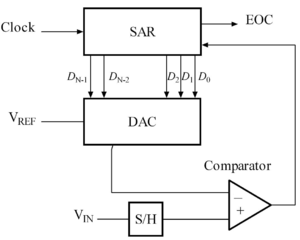
\includegraphics[width=8cm]{sar_adc.png}
% 	\caption{\ac{SAR}}
% \end{figure}

\subsubsection{Ultrasonický senzor HC-SR04}

\ac{HC-SR04} vydává zvukové vibrace na vysoké frekvenci, neslyšitelné pro lidské ucho. Poté čeká, až se zvuk odrazí zpět od překážky, a vypočítá vzdálenost na základě času měřeného od vysílání zvukové vlny k zpětnému přijmutí

Všechny naměřené údaje jsou v převodníku senzoru přepočítány a odeslány analogovým signálem do řídící jednotky.
% TODO: převodník nepřepočítává hovno, za jak dlouho se zvuk vrátí počítá code

\subsubsection{Čerpadlo}

Naše zvolené ponorné mini čerpadlo eses se skládá z DC motoru, na němž je upevněna centrifuga pro čerpání vody a vlastního pouzdra, z kterého vede otvor pro napojení odtokové hadičky. Čerpadlo je připojeno na zdroj napětí 5V a zem.

\subsubsection{Tranzistor 2N2222}

Protože samotný signální pin neposkytuje dostatečné napětí pro chod čerpadla ovládáme jej tranzistorem 2N2222. Tento tranzistor je bipolární Negative-Positive-Negative tranzistor, to znamená že jeho polarita je nastavená tak aby na kolektoru přijímal pozitivní napětí. Díky našemu vyměnitelnému připojení modulů je možné čerpadlo vyměnit za jiné a přívodný kabel používat jako spouštěč čerpadla jakéhokoliv výkonu a nároků na zdroj.

\subsection{Architektura ARM}

\ac{ARM} je založen na Reduced Instruction Set Computing (RISC) a je to nejnověji používaná CPU architektura. Tyto procesory jsou designované na všechny moderní chytré telefony, zařízení s operačním systémem Android i Apple produkty.

\clearpage

\section{Návrh obvodu a plošného spoje}

Testovací verzi našeho obvodu jsme postavili na nepájivém kontaktním poli. Jakmile jsme měli vše plně odzkoušeno a plně otestováno, přešli jsme na profesionálnější řešení. Což tedy v druhé fázi znamenalo navrhnout a nechat vytisknout náš vlastní obvod přepracovaného schématu \ac{PCB} a vytisknutého společností JLCPCB na naše vlastní náklady.

\begin{figure}[h]
	\centering
	\begin{subfigure}[b]{0.4\linewidth}
		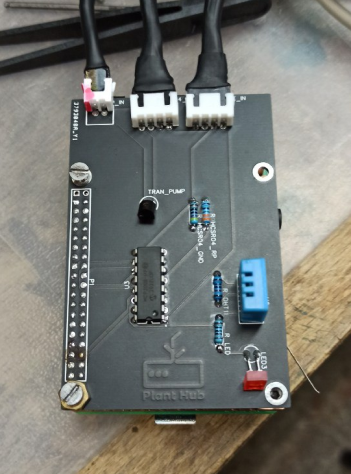
\includegraphics[width=\linewidth]{pcb.png}
		\caption{Diagram \ac{PCB}}
	\end{subfigure}
	\begin{subfigure}[b]{0.4\linewidth}
		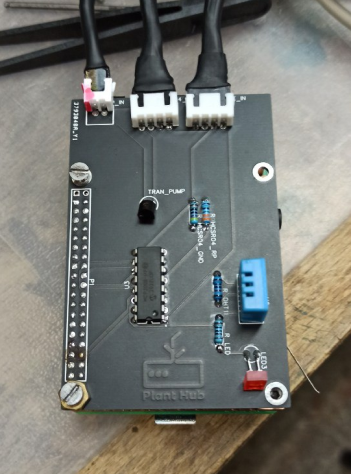
\includegraphics[width=\linewidth]{planthub.png}
		\caption{PlantHub \ac{PCB} se senzory}
	\end{subfigure}
	\caption{}
\end{figure}

\clearpage

\section{Fyzická realizace}

% předělat na fotku celého planthubu

\begin{figure}[h]
	\centering
	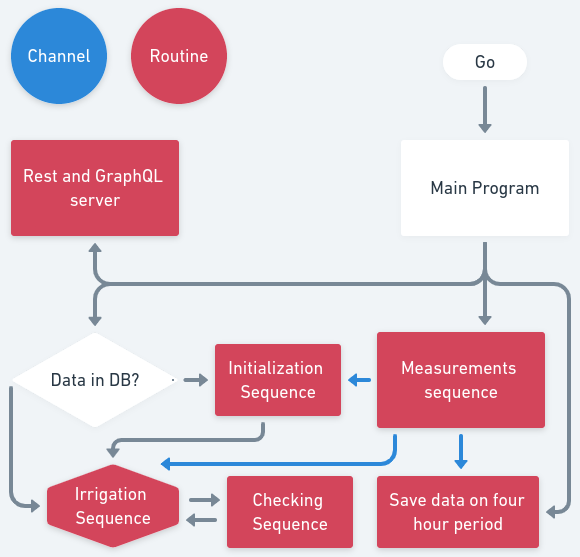
\includegraphics[width=0.72\linewidth]{go.png}
	\caption{Fyzická realizace}
\end{figure}

\clearpage

\section{Hlavní program}

\subsection{Postup práce}

Náš hlavní program pro zavlažování a komunikaci s databází a \ac{WUI} jsme začali psát ve vysokoúrovňovém programovacím jazyce Python. Od toho jsme ale nakonec upustili kvůli horší výkonu, a tak jsme program přepsali v programovacím jazyku Go.

\begin{figure}[h]
	\centering
	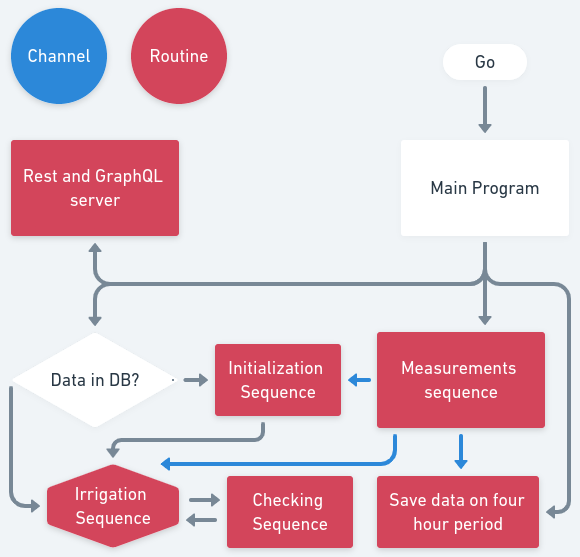
\includegraphics[width=0.72\linewidth]{go.png}
	\caption{Vývojový diagram programu}
\end{figure}

\subsection{Fáze programu}

Fáze programu se spouštějí buďto v samostatné go rutině a komunikují spolu pomocí kanálů nebo na základě podmínek, kde se po splnění požadavků ukončí.

\subsubsection{Měření}

Senzor vlhkosti půdy a \ac{DHT11} průběžně posílají naměřená data do \ac{RPi}, kde se ukládají do databáze. Jestliže naměřené hodnoty překročí limitní hodnoty, \ac{RPi} pošle signál pro otevření tranzistoru což spustí čerpadlo.

% TODO: více rozvést vliv obou senzorů

\subsubsection{Periodické ukládání dat}

V samostatné rutině běží funkce pro ukládání naměřených dat v periodě 4 hodin. Naměřená data jsou následně statisticky zobrazena v \ac{WUI}.

\subsubsection{Controller}

Po spuštění měřící sekvence a sekvence periodického ukládání dat se spustí buďto inicializační sekvence a nebo zavlažovací sekvence podle toho, jestli se v databázi nachází předchozí nastavení. Pokud předchozí nastavení nejsou nalezena, program čeká na uložení dat z \ac{WUI} a \ac{LED} dioda bliká dvakrát po sobě, dokud data nejsou dostupná. Pokud jsou, spustí se zavlažovací sekvence, načtou se limitní data z databáze a v periodě jedné sekundy se budou číst data o vlhkosti půdy.

\subsubsection{Inicializace}

Půda musí být ze začátku suchá. Senzor vlhkosti půdy zasuneme co nejhlouběji do půdy. \ac{RPi} bude chvíli sbírat data a pak je zprůměruje do hodnoty, která bude sloužit jako limit pro spuštění čerpadla.

V \ac{WUI} jde navíc ještě manuálně nastavit hranice vlhkosti půdy pro spuštění
čerpadla.

Nastavit se dá také množství vody, které bude přečerpáno při jednom spuštění a jaká je hranice pro přijatelnou výšku hladiny vody v nádrži. Pokud nejsou tyto hodnoty uvedeny čerpadlo bude vodu přečerpávat, dokud se nezmění hodnota kapacitního čidla pro měření vlhkosti půdy a \ac{HC-SR04} použije výchozí nastavení.

\subsubsection{Zavlažování}

Čerpadlo začne čerpat vodu a zavlažovat rostlinu. Voda se čerpá tak dlouho, dokud senzor vlhkosti půdy nezmění svou hodnotu nebo dokud není vyčerpán limit přečerpané vody na jedno spuštění.

\subsubsection{Kontrola}

Po ukončení přečerpávání se spustí \ac{HC-SR04} a změří výšku hladiny vody. Naměřená data poté odešle do \ac{RPi} kde se uloží do databáze. Pokud bude naměřená hodnota nižší, než je limitní hodnota, začne blikat \ac{LED} a \ac{RPi} odešle upozornění o doplnění nádrže do \ac{WUI}. Jakmile bude hladina doplněna, signalizace se vypne.

\subsubsection{Ukládání dat}

Náš systém ukládá zvlášť periodicky naměřená data a data naměřená před zavlažováním, dále ukládá nastavení jak pro limity k zavlažování, tak pro \ac{WUI}.

\subsection{Go}

Go je open-source programovací jazyk, který byl vytvořen společností Google v roce 2009. Je to stále relativně nový programovací jazyk, který se nevyvinul z jiných jazyků jako C\# a Java. Go ignoruje teorii o programovacích jazycích. Místo toho aby se zaměřoval na akademické teorie, se zaměřuje na reálné praktiky používané pro vývoj next-gen v cloudových, distribuovaných a souběžných aplikacích.

Jazyk Go je staticky typovaný a využívá garbage collector, jedná se o kompilovaný programovací jazyk, který své binární soubory kompiluje pro každou platformu. Dá se zařadit do skupiny C jazyků na základě jeho základního syntaxe. Go poskytuje expresivní syntax s jednoduchým typovým systémem a má vestavěné nástroje pro paralelní programování. Výkon Go je srovnatelný s jazyky C a C++, ale zároveň nabízí rychlý a jednoduchý vývoj aplikací.

Stejně jako C a C++ se Go kompiluje do nativního strojového kódu, takže
nepotřebujeme běhové prostředí jako Common Language Runtime (CLR) a Java Virtual Machine (JVM). To má řadu výhod, třeba při distribuci aplikace v aplikačních kontejnerech jako je Docker.

\subsubsection{Paralelní programování v Go}

Vývoj počítačů se v průběhu posledního desetiletí značně posunul. V minulosti aplikace běžely na počítačích pouze s jediným procesorovým jádrem. Dnes je standardní vidět čtyřjádrové procesory v uživatelských počítačích, dokonce i naše Raspberry má dvě jádra. Stále ale používáme programovací jazyky a technologie navržené v éře, kdy byly dostupné pouze jednojádrové procesory.

Většina programovacích jazyků dnes nabízí knihovny nebo frameworky pro \linebreak paralelní programování, ale nemají tuto vlastnost zbudovanou přímo v jádře jazyka. V Go je paralelní programování součástí jazyka už od samotného počátku. Používá takzvané Gorutiny, které umožňují spouštět funkce souběžně. Souběžné funkce pak mezi sebou mohou komunikovat a předávat data pomocí kanálů. Dokonce i některé standardní knihovny jazyka mají zabudovanou souběžnost. Například standardní knihovna `net/http' pro programování HTTP zpracovává přicházející požadavky souběžně pomocí Gorutin.

\subsubsection{Typový systém}

Pragmatický design Go neobsahuje klíčové slovo pro třídu a jeho objektová orientace je odlišná od tradičních objektově orientovaných programovacích jazyků. V Go nahrazuje funkci tradiční třídy typ struct. Dědění není v go podporováno, ale podporuje kompozici typů.

Zde je příklad, který demonstruje typový systém Go spolu s rozhraním (interface), typem struct a vnořením pro typovou kompozici.

%Ukázka typového systému

\clearpage


\section{WUI}

Webovovou aplikaci jsme napsali pomocí javascriptového frameworku
React.js, CSS frameworku Tailwind a programovacího jazyku Typescript, který je supersetem javascriptu, podporujícím volitelné statické typování. Ve webovém rozhraní je možné zobrazit
si statisky jak živě naměřených dat, tak dat uložených v databázi. Z OpenWeather \ac{API} získáváme data o předpovědi počasí a do dahsboardu renderujeme předpovědi na dalších 15H.

\begin{figure}[h]
	\centering
	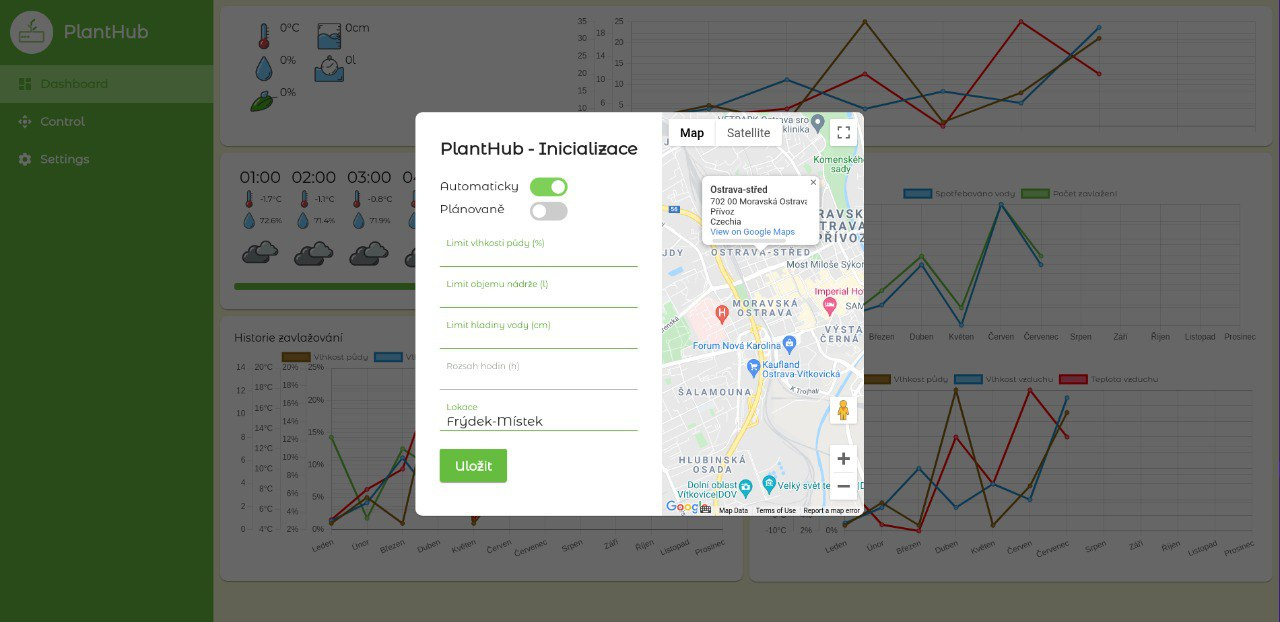
\includegraphics[width=\linewidth]{ui-inicializace.jpg}
	\caption{Okno prvotního nastavení. Nastaví se zde limity a celkové
		nastavení aplikace.}
\end{figure}

\begin{figure}[h]
	\centering
	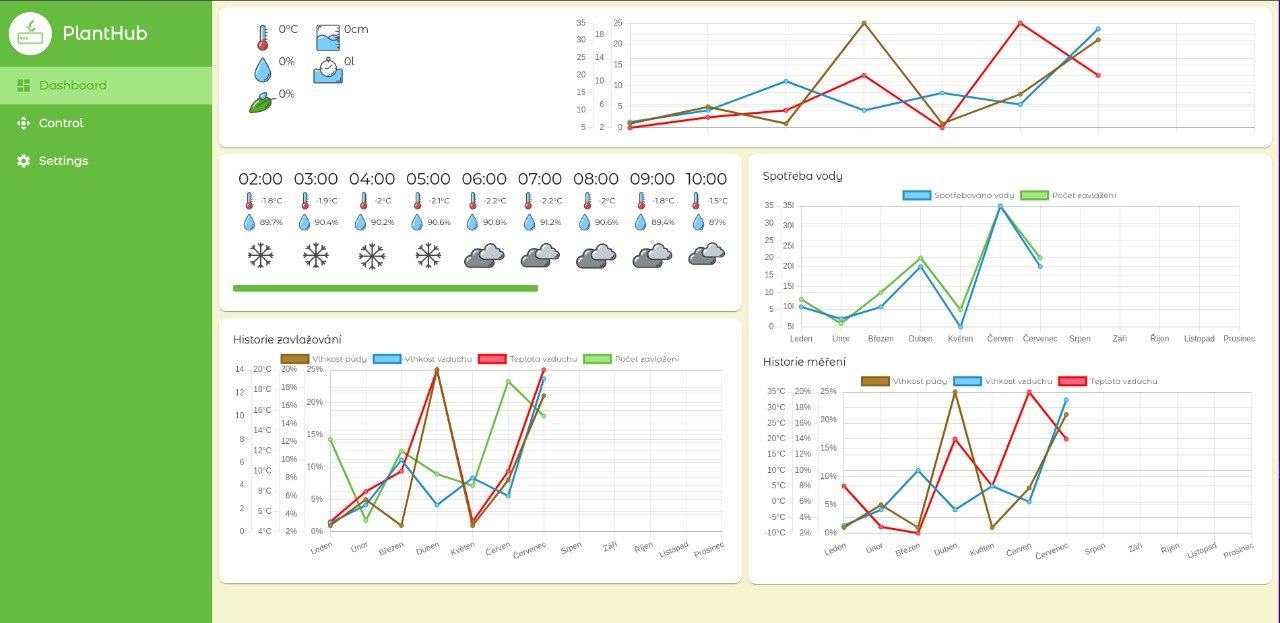
\includegraphics[width=\linewidth]{web-ui.png}
	\caption{Dashborad \ac{WUI}}
\end{figure}

\begin{figure}[h]
	\centering
	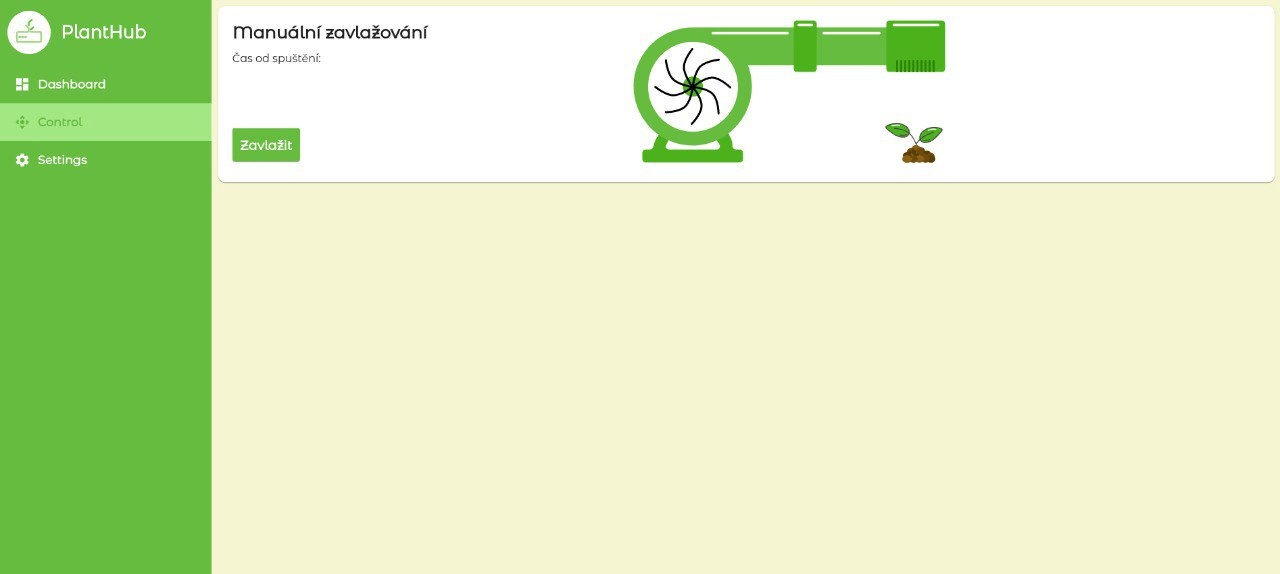
\includegraphics[width=\linewidth]{web-ui-pump.png}
	\caption{Interaktivní ovládání celého systému lze provést v již
		zmiňované webové aplikaci. Dovoluje uživateli kdykoliv spustit
		čerpadlo na
		zalévání rostliny.}
\end{figure}

\begin{figure}[h]
	\centering
	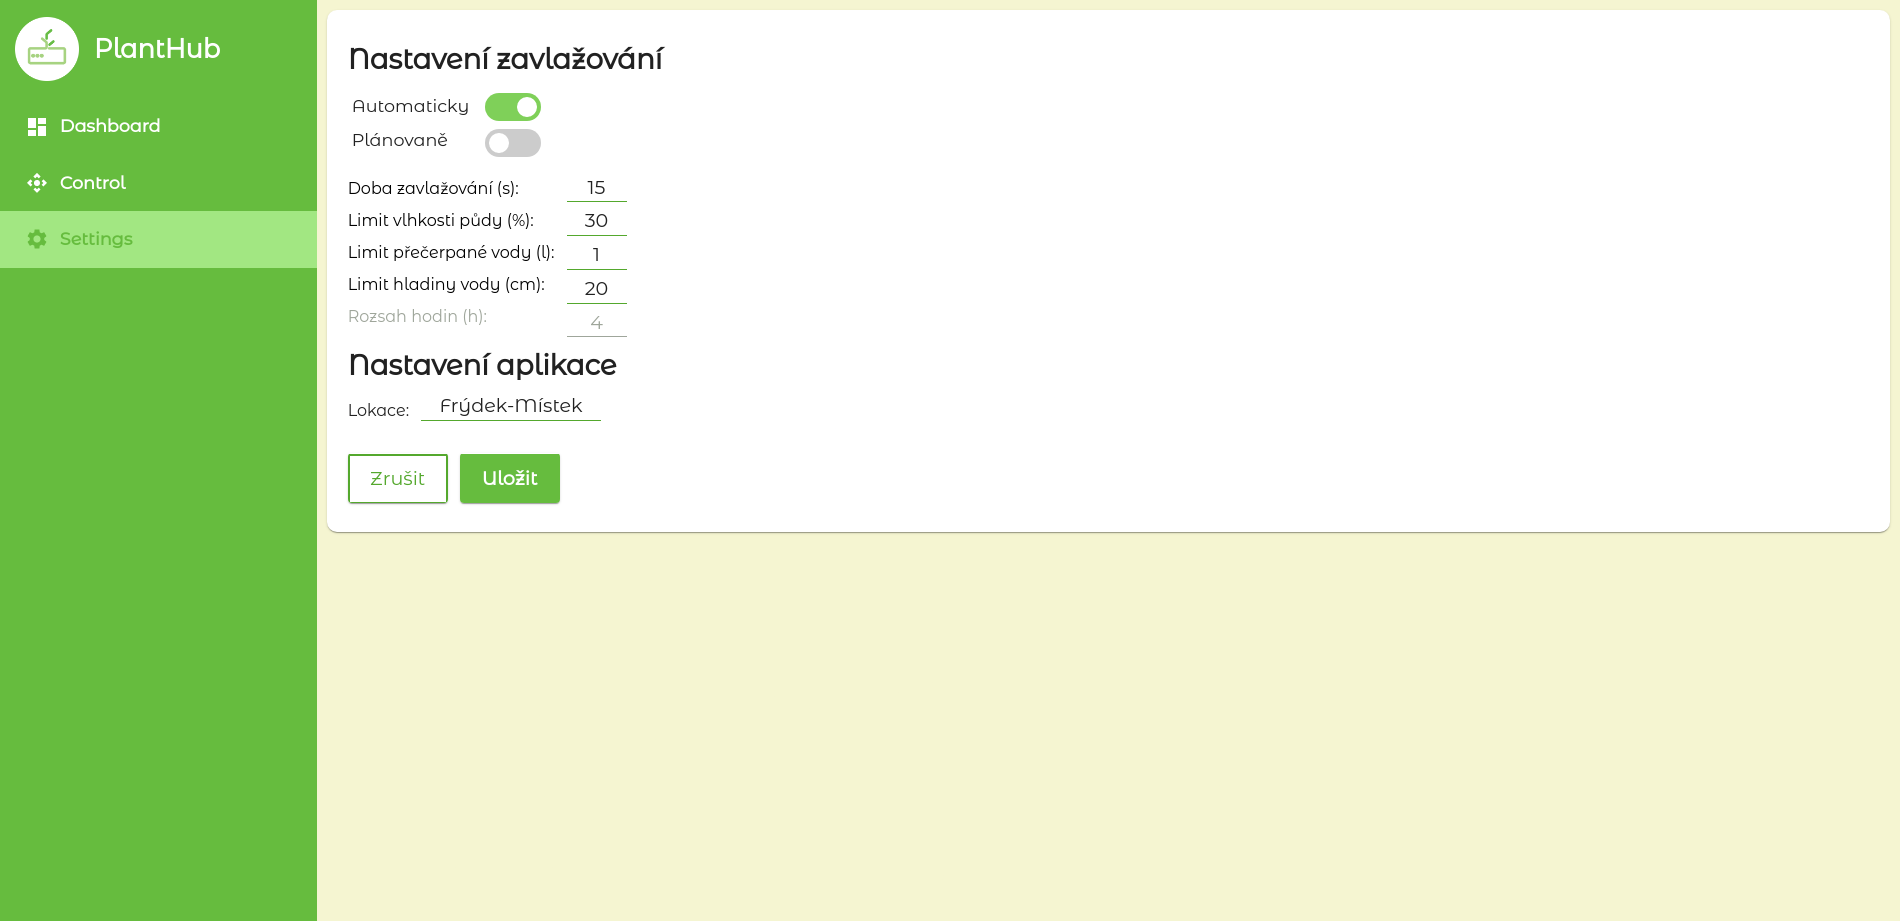
\includegraphics[width=\linewidth]{web-ui-settings.png}
	\caption{V nastavení se dá změnit nastavení aplikace i limitů pro
		zavlažování. Nastavení se poté uloží do databáze.}
\end{figure}

\clearpage

\section{Databáze}

Pro databázi jsme se rozhodli použít databázový systém PostgreSQL.\@ Jak vyplývá z názvu, jedná se o Structured Query Language (SQL) databázi, ty jsou vhodné pro ukládání velkého objemu dat, jako právě data z našich senzorů. Webová aplikace používá pro přístup k datům z databáze GraphQL \ac{API}.\@

GraphQL je query, který je konkurent řešení \ac{REST} \ac{API}.\@ Nabízí rychlejší
tvorbu \ac{API} a také umožňuje efektivnější přístup k datům z databáze. Umožňuje
vybrat pouze data, která momentálně aplikace používá a dovoluje vynechat data,
která zrovna potřebné nejsou.

\begin{figure}[h]
	\centering
	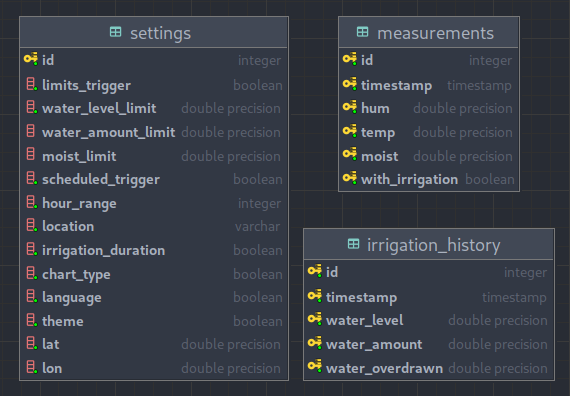
\includegraphics[width=0.9\linewidth]{db.png}
	\caption{Schéma databáze}
\end{figure}

\section{Webový server}

Web server jsme napsali v moderním jazyku Go, který nyní roste v popularitě hlavně mezi cloudovými vývojáři a v oblasti vývoje microservices. Dokáže se v rychlosti provedení programu přiblížit k nízkoúrovňovým jazykům jako je C nebo Rust, ale zároveň zůstává velmi lidsky čitelný a jednoduchý na použití. Na rozdíl od jazyků jako C a Rust má například garbage collector, který periodicky čistí paměť a zabraňuje memory leakům.

\section{Bezpečnost}

\section{Závěr}

Náš projekt je stále ve vývoji a mnoho z kritických funkcí projektu není ještě dokončeno. S vývojem dále pokračujeme, protože se jedná o naši maturitní práci. Myslíme si, ale že tento projekt má v budoucnu potenciál stát se úspěšným startupem, proto plánujeme pokračovat ve vývoji i po maturitě.

Tato práce byla pro nás velkým přínosem, naučili jsme se mnoho nových dovedností a načerpali nové informace.

% TODO: co zbývá dokončit?
% TODO: Budoucí plány

\clearpage

\section{Použitá literatura další zdroje }

\begin{thebibliography}{9}
	\vspace*{-1.5cm}
	\bibitem{texbook}
	“Home,” LaTeX, 06-May-2021. [Online]. Available: \href{https://latex-tutorial.com/}{https://latex-tutorial.com/}. [Zpřístupněno: 10-Dubna-2022]. 

	\bibitem{golang}
	“Build fast, reliable, and efficient software at scale,” Go. [Online]. Dostupné z: \href{https://go.dev/}{https://go.dev/}. [Zpřístupněno: 10-Dubna-2022]. 

	\bibitem{react}
	“React – a JavaScript library for building user interfaces,” – A JavaScript library for building user interfaces. [Online]. Available: \href{https://reactjs.org/}{https://reactjs.org/}. [Zpřístupněno: 10-Dubna-2022]. 

	\bibitem{tailwindcss}
	“Rapidly build modern websites without ever leaving your HTML.,” Tailwind CSS. [Online]. Available: \href{http://www.tailwindcss.com/}{http://www.tailwindcss.com/}. [Zpřístupněno: 10-Dubna-2022]. 

	\bibitem{typescript}
	“JavaScript with syntax for types.,” TypeScript. [Online]. Available: \href{http://www.typescriptlang.org/}{http://www.typescriptlang.org/}. [Zpřístupněno: 10-Dubna-2022]. 

	\bibitem{vscode}
	Microsoft, “Visual studio code - code editing. redefined,” RSS, 03-Nov-2021. [Online]. Available: \href{https://code.visualstudio.com/}{https://code.visualstudio.com/}. [Zpřístupněno: 10-Dubna-2022]. 

	\bibitem{goland}
	“Goland by jetbrains: More than just A go ide,” JetBrains. [Online]. Available: \href{https://www.jetbrains.com/go/}{https://www.jetbrains.com/go/}. [Zpřístupněno: 10-Dubna-2022]. 

	\bibitem{git}
	Git. [Online]. Available: \href{https://git-scm.com/}{https://git-scm.com/}. [Zpřístupněno: 10-Dubna-2022]. 

	\bibitem{figma}
	“The Collaborative Interface Design Tool.,” Figma. [Online]. Available: \href{https://www.figma.com/}{https://www.figma.com/}. [Zpřístupněno: 10-Dubna-2022]. 

	\bibitem{freecad}
	“Freecad,” FreeCAD. [Online]. Available: \href{https://www.freecadweb.org/}{https://www.freecadweb.org/}. [Zpřístupněno: 10-Dubna-2022]. 

	\bibitem{easyeda}
	Supplyframe, “EasyEDA,” Component Search Engine. [Online]. Available: \href{https://componentsearchengine.com/library/easyeda}{https://componentsearchengine.com/library/easyeda}. [Zpřístupněno: 10-Dubna-2022]. 
\end{thebibliography}

\section{Seznam příloh}

\begin{itemize}
	\item \href{https://github.com/POJFM/dmp-plant-hub}{Zdrojový kód, dostupný na github.com/POJFM/dmp-plant-hub}
	\item Prezentace
	\item \href{https://www.youtube.com/watch?v=oo2_pDX5OE4}{Videoprezentace, dostupná na youtube.com}
\end{itemize}

\end{document}